\section{Media Management S3 Component}
\label{sec:S3_component}

In this section will be analyzed the Media Management S3 Component, developed to store images and documents on cloud through Amazon S3 Service.
This specific component has been developed in order to store and manage media files in Amazon S3 service.
Operations that can be done, like upload, delete or get media, is ruled by CORS (\ref{subsec:S3_cors}) pattern.
These operations are direct: none of them is done via server. Server is only used to get the authorization to communicate with the S3 cloud storage service.
In fact, client makes an AJAX request to server in order to get the Signed URL, that is the request URL combined with the name of S3 Bucket and the dedicated Region.
The Signed URL pattern represents the Digital Signature security mechanism, as seen in \ref{sec:digsign}.

The Signed URL is requested via an ad hoc API, that is exposed to client side through a remote method.
Get, Upload and Delete functions have been implemented on the server side using an additional library named AWS SDK for Javascript NodeJS \footnote{ The AWS SDK helps take the complexity out of coding by providing JavaScript objects for AWS services including Amazon S3, Amazon EC2, DynamoDB, and Amazon SWF.} \cite{s3_aws_sdk}.

Each function create a request for a Signed URL to its server.
Using file's name, bucket's name, bucket's region and user key, the server gives back an URL to which the client can his real HTTP request.

Once the client receive the Signed URL can pass the operation to S3 Service and carry it out.
Bucket and Region names are stored in \texttt{.env} file and must be set up before on S3 website.
Moreover, users must set Bucket's CORS Configuration on S3 Admin Panel: CRUD operations must be allowed from the user in the CORS Configuration Editor panel.


\subsubsection{Upload Signed Url Request}

\begin{lstlisting}[language=javascript]
Image.signed_put = function(file_name, file_type, callback) {
    var s3 = new aws.S3();
    var s3_params = {
      Bucket: S3_BUCKET,
      Key: file_name,
      Expires: 60,
      ContentType: file_type,
      ACL: 'public-read'
    };
    s3.getSignedUrl('putObject', s3_params,
     function (err, signed_url) {
      if (err) {
        callback(err);
        return;
      }
      callback(null, signed_url);
    });
  };

  Image.remoteMethod('signed_put', {
    http: { verb: 'get' },
    accepts: [
      {arg: 'file_name', type: 'string'},
      {arg: 'file_type', type: 'string'}
    ],
    returns: {arg: 'signed_url', type: 'string'}
  });
\end{lstlisting}

\subsubsection{Get Signed Url Request}

\begin{lstlisting}[language=javascript]
Image.signed_list = function (folder, callback) {
    var s3 = new aws.S3();
    var s3_params = {
      Bucket: S3_BUCKET,
      EncodingType: 'url',
      Prefix: folder,
      MaxKeys: 1000
    };
    s3.getSignedUrl('listObjects', s3_params,
     function (err, signed_url) {
      if (err) {
        callback(err);
        return;
      }
      callback(null, signed_url);
    });
  };

  Image.remoteMethod('signed_list', {
    http: { verb: 'get' },
    accepts: { arg: 'folder', type: 'string' },
    returns: { arg: 'signed_url', type: 'string' }
  });
\end{lstlisting}


\subsubsection{Delete Signed Url Request}

\begin{lstlisting}[language=javascript]
Image.signed_delete = function(file_name, callback) {
    var s3 = new aws.S3();
    var s3_params = {
      Bucket: S3_BUCKET,
      Key: file_name
    };
    s3.getSignedUrl('deleteObject', s3_params,
      function (err, signed_url) {
      if (err) {
        callback(err);
        return;
      }
      callback(null, signed_url);
    });
  };

  Image.remoteMethod('signed_delete', {
    http: { verb: 'get' },
    accepts: {arg: 'file_name', type: 'string'},
    returns: {arg: 'signed_url', type: 'string'}
  });

\end{lstlisting}


\begin {figure}[h]
\graphicspath{{images/chapter_s3/}}
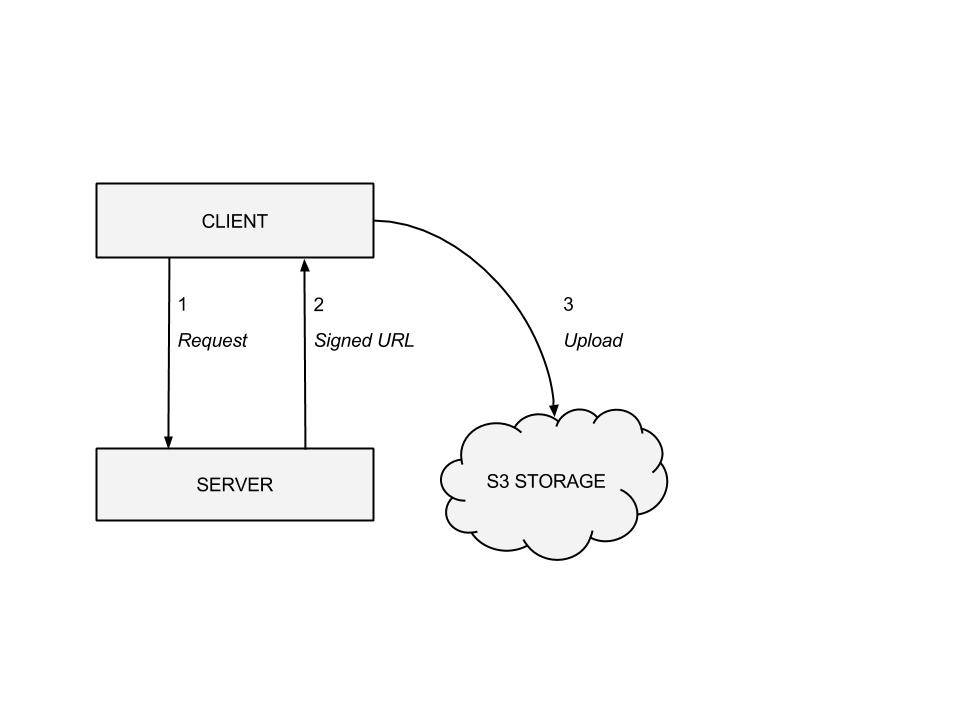
\includegraphics[width=\textwidth]{s3_upload}
\caption{S3 direct upload process}
\end {figure}



\begin {figure}[h]
\graphicspath{{images/chapter_s3/}}
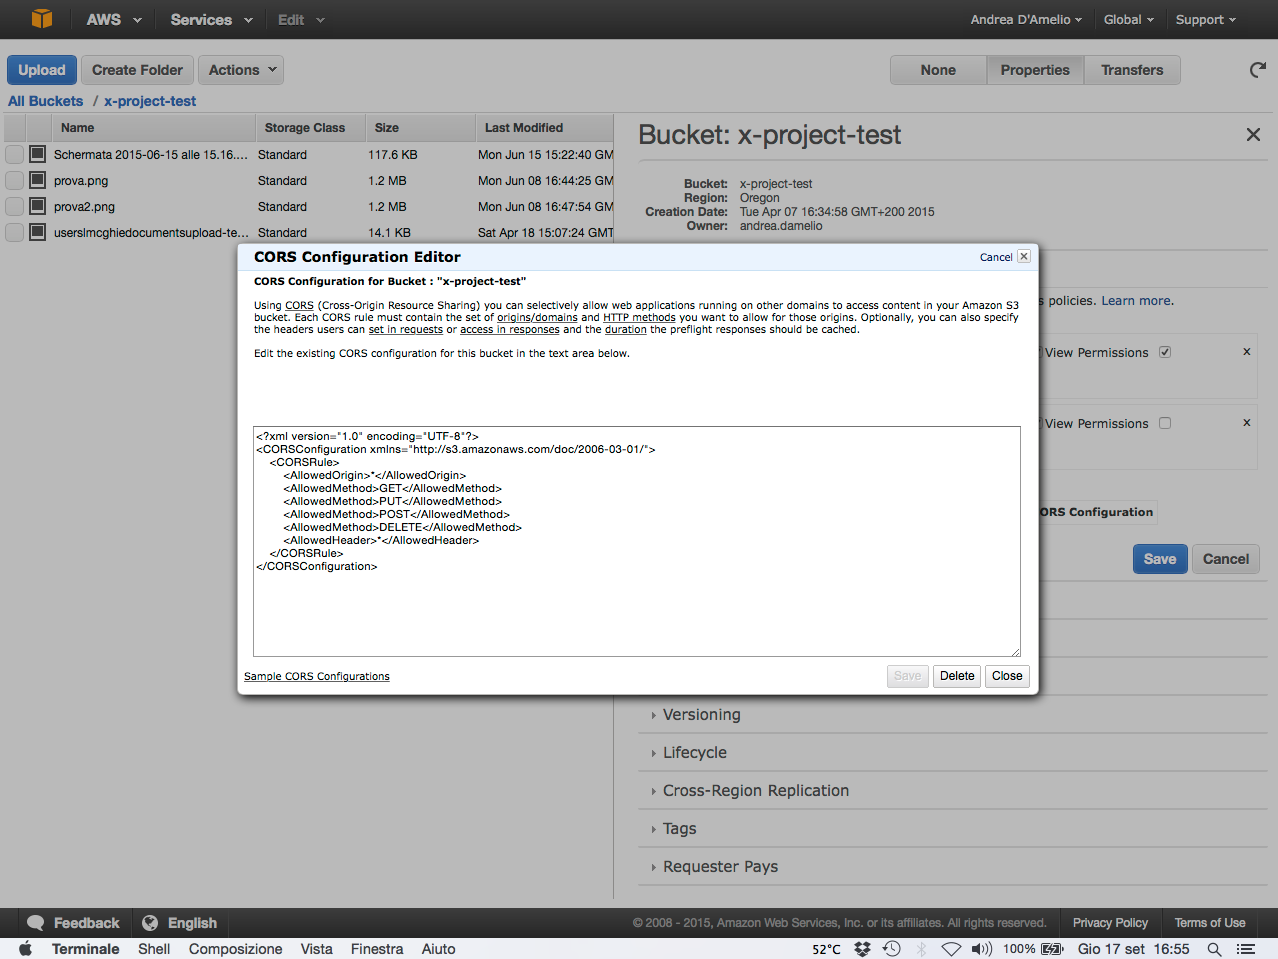
\includegraphics[width=\textwidth]{s3panel}
\caption{S3 CORS Configuration Editor Panel}
\end {figure}









\subsection{S3 Component Elements}
\label{subsec:S3_server_elem}


In order to use Media Management S3 Component in an X-Project App there's need to combinate six different X-Elements:
\begin{itemize}

\item\texttt{api-s3-upload},
\item\texttt{api-s3-list},
\item\texttt{api-s3-delete},
\item\texttt{part-s3-list},
\item\texttt{part-s3-list-item}
\item\texttt{part-s3-upload}.

\end{itemize}

Each element provides the opportunity to use one of the basic function of Amazon S3 service. 

\subsubsection{\texttt{api-s3-upload}}
\label{api-s3-upload}


The element named \texttt{api-s3-upload} has been designed to upload new files to the S3 Bucket.
\begin{lstlisting}[language=javascript]
<api-s3-upload id="upload" folder="{{folder}}"
	file="{{file}}" file-name="{{fileName}}">
</api-s3-upload>
\end{lstlisting}


\subsubsection{\texttt{api-s3-list}}
\label{api-s3-list}
The element named \texttt{api-s3-list} has been designed to get the list of elements currently in the S3 Bucket.
\begin{lstlisting}[language=javascript]
<api-s3-list id="list" list="{{list}}">
</api-s3-list>
\end{lstlisting}


\subsubsection{\texttt{api-s3-delete}}
\label{api-s3-delete}
The element named \texttt{api-s3-delete} has been designed to delete an element currently in the S3 Bucket.
\begin{lstlisting}[language=javascript]
<api-s3-delete id="request" file-name="{{item.key}}">
</api-s3-delete>
\end{lstlisting}


\subsubsection{\texttt{part-s3-list}}
\label{part-s3-list}
The element named \texttt{part-s3-list} has been developed to show the list of elements currently in the S3 Bucket
\begin{lstlisting}[language=html]
<template>
    <api-s3-list id="list" list="{{list}}">
    </api-s3-list>

    <template is="dom-repeat" items="{{list}}" filter="filter">
        <part-s3-list-item item="{{item}}" on-delete="update">
        </part-s3-list-item>
    </template>
</template>
\end{lstlisting}
The first tag, \texttt{<api-s3-list>}, calls the GET API that handles the request to S3, and returns the list of elements currently in S3 Bucket.
The second tag, \texttt{<part-s3-list-item>}, creates a visual element for each object currently in the bucket. This cycle is expressed via the attribute \texttt{``dom-repeat''}.


\subsubsection{\texttt{part-s3-list-item}}
\label{part-s3-list-item}
The element named \texttt{part-s3-list-item} has been developed to show a preview of a selected files and to let the user delete it.
\begin{lstlisting}[language=javascript]

 <api-s3-delete id="request" file-name="{{item.key}}">
 </api-s3-delete>
 ...
 <button id="delete" on-click="delete_image">delete
 </button>
 ...
 delete_image: function () {
      this.$.request.send();
 }
 ...
\end{lstlisting}

The first tag, \texttt{<api-s3-delete>}, set the DELETE API that handles the request to S3.
The button tag creates a button that, when clicked, trigger the \texttt{delete image} function, that makes the call via \texttt{<api-s3-delete>} element.


\subsubsection{\texttt{part-s3-upload}}
\label{part-s3-upload}
The element named \texttt{part-s3-upload} has been developed to allow to users to upload new files to the S3 Bucket.

\begin{lstlisting}[language=javascript]
<api-s3-upload id="upload"
      file="{{file}}" file-name="{{fileName}}">
</api-s3-upload>

<input id="input" type="file" on-change="on_change">
on_change: function () {
      var file = this.$.input.files[0];
      if (!file) {
        return;
      }
      this.fileName = this.fileName || file.name;
      this.file = file;
    }

\end{lstlisting}

The first tag, \texttt{<api-s3-upload>}, set the upload API that handles the request to S3.
The input tag creates a input form that let the user choice the file to upload and trigger the \texttt{on change} function, that send the file via \texttt{<api-s3-upload>} element.
